\documentclass{beamer}
\usepackage{relsize}
\usepackage{color}

\usepackage{listings}
\usetheme{CambridgeUS}
%\usepackage{beamerthemesplit} % new
\usepackage{enumitem}
\usepackage{amsmath}                    % See geometry.pdf to learn the layout options.
\usepackage{amsthm}                   % See geometry.pdf to learn the layout options. There
\usepackage{amssymb}                    % See geometry.pdf to learn the layout options.
\usepackage[utf8]{inputenc}
\usepackage{graphicx}
\usepackage[english,bulgarian]{babel}

\usepackage{caption}
\usepackage{tikz}

\usetheme{CambridgeUS}
\usecolortheme{crane}

\lstset{language=C++,
                basicstyle=\ttfamily,
                keywordstyle=\color{blue}\ttfamily,
                stringstyle=\color{red}\ttfamily,
                commentstyle=\color{green}\ttfamily,
                morecomment=[l][\color{magenta}]{\#}
}

\newtheorem{mydef}{Дефиниция}[section]
\newtheorem{lem}{Лема}[section]
\newtheorem{thm}{Твърдение}[section]

\DeclareMathOperator{\restrict}{\upharpoonright}

\setitemize{label=\usebeamerfont*{itemize item}%
  \usebeamercolor[fg]{itemize item}
  \usebeamertemplate{itemize item}}

\setbeamercovered{transparent}

\captionsetup{font=tiny} 

\begin{document}
\title[Монади]{Монади. Практически поглед}
\frame{\titlepage}

\section{Монади}
\subsection{Maybe}


\begin{frame}[fragile]
  \frametitle{Състояние}

\begin{lstlisting}[basicstyle=\small,language=Haskell]
type Pos = (Int, Int)
  
data Tile = Road | Wall | Gold
            deriving (Show, Eq)
  
data Game = Game { pos :: Pos, world :: [[Tile]]}
            deriving (Show)
  
myWorld :: Game = Game { pos = (0, 0), 
                         world = [[Road, Wall, Gold], 
                                  [Road, Wall, Road], 
                                  [Road, Road, Road]]}
\end{lstlisting}

\begin{tikzpicture}[remember picture,overlay]
  \node[xshift=75mm,yshift=-12mm,anchor=north west] at (current page.north west){%
  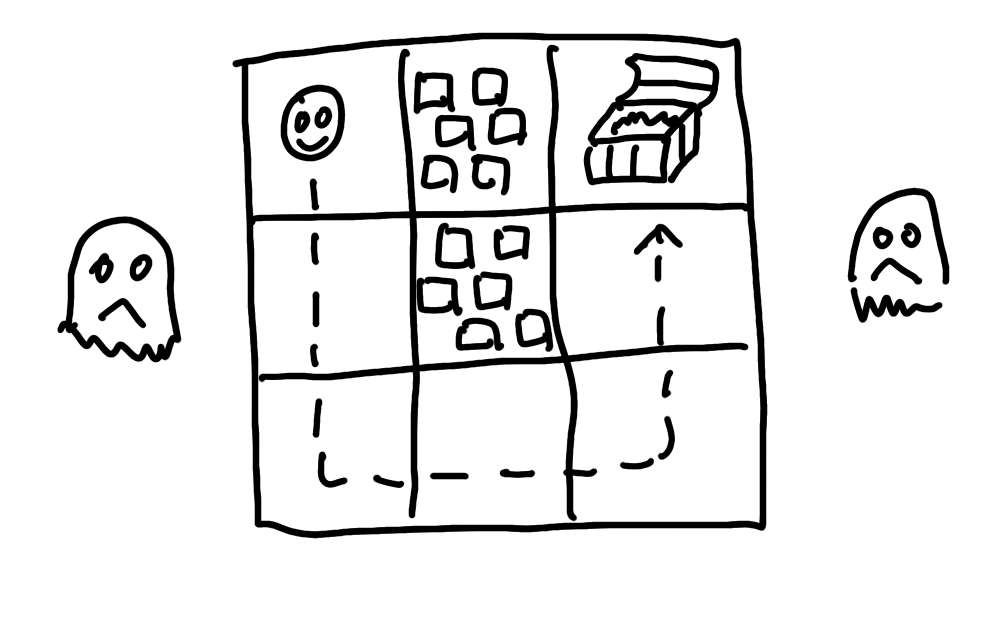
\includegraphics[width=50mm]{images/maze.png}};
\end{tikzpicture}

\end{frame}


\begin{frame}[fragile]
  \frametitle{Операции}

\begin{lstlisting}[basicstyle=\small,language=Haskell]
left (Game (x, y) w) = Game (x-1, y) w
right (Game (x, y) w) = Game (x+1, y) w
up (Game (x, y) w) = Game (x, y-1) w
down (Game (x, y) w) = Game (x, y+1) w
\end{lstlisting}

\end{frame}


\begin{frame}[fragile]
  \frametitle{Композиране на операции}

\begin{lstlisting}[basicstyle=\small,language=Haskell]
walk1 g = (up . up . right . right . down . down) g
\end{lstlisting}

\begin{tikzpicture}[remember picture,overlay]
  \node[xshift=75mm,yshift=-12mm,anchor=north west] at (current page.north west){%
  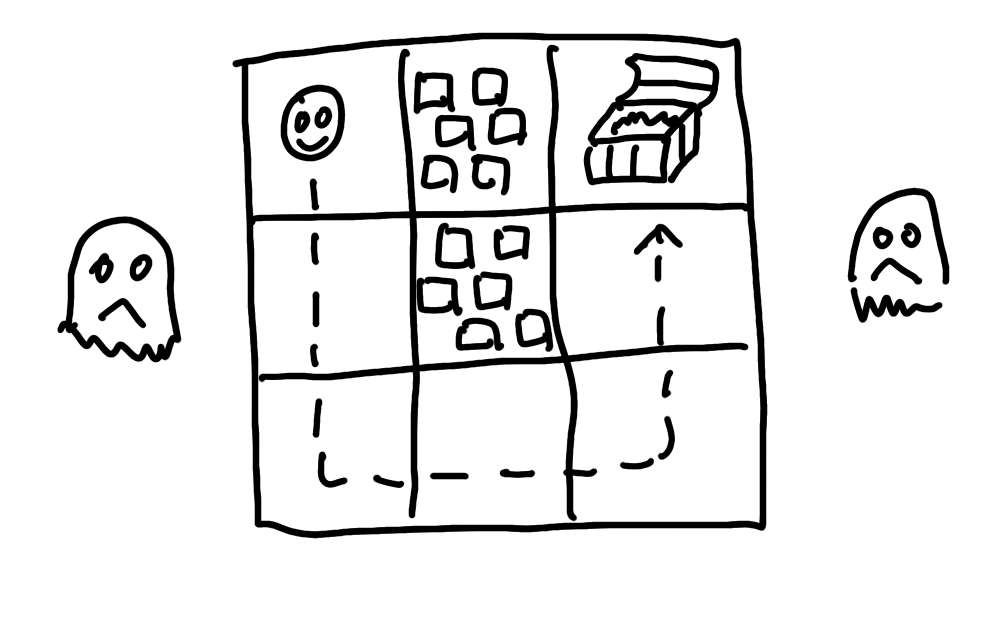
\includegraphics[width=50mm]{images/maze.png}};
\end{tikzpicture}


\end{frame}


\begin{frame}[fragile]
  \frametitle{Композиране на операции}

\bigskip
\bigskip
\bigskip
\bigskip
\bigskip

\begin{lstlisting}[basicstyle=\small,language=Haskell]
walk1 = up . up . right . right . down . down

(->>) :: Game -> (Game->Game) -> Game
g ->> f = f g

walk1 g = g->>down->>down->>right->>right->>up->>up
\end{lstlisting}

\begin{tikzpicture}[remember picture,overlay]
  \node[xshift=75mm,yshift=-12mm,anchor=north west] at (current page.north west){%
  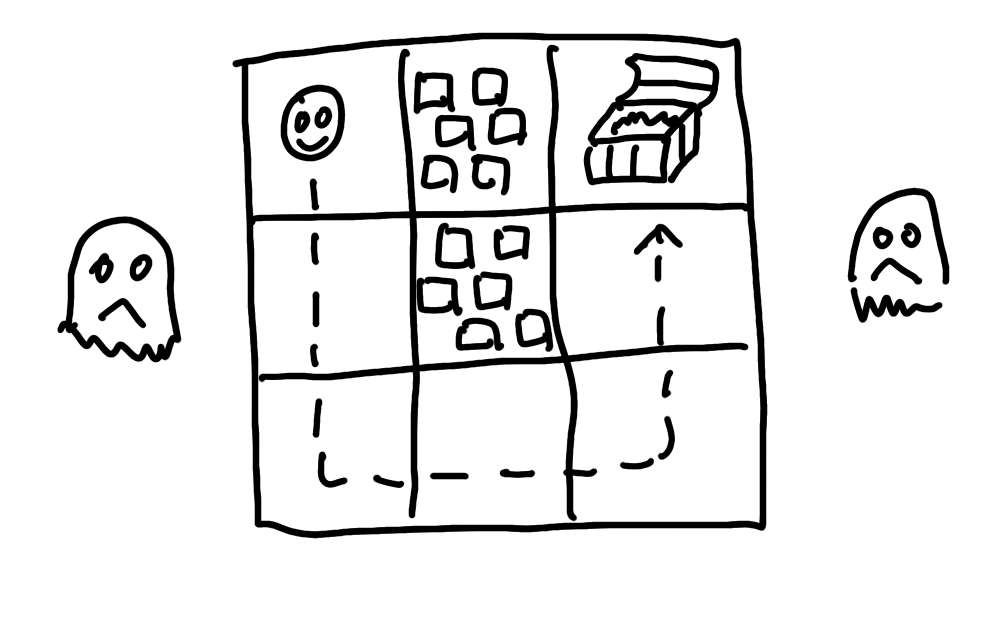
\includegraphics[width=50mm]{images/maze.png}};
\end{tikzpicture}

\end{frame}


\begin{frame}[fragile]
  \frametitle{Грешки}

\begin{lstlisting}[basicstyle=\small,language=Haskell]
dead :: [[Tile]] -> Pos -> Bool
dead w (x, y) = x < 0 || x >= length w ||
                y < 0 || y >= length w || 
                (w !! y) !! x == Wall

left (Game (x, y) w) 
    | dead w (x-1,y) = error "Error, dead player!"
    | otherwise = Game (x-1, y) w

ghci> left myWorld 
*** Exception: Error, dead player!
\end{lstlisting}


\begin{tikzpicture}[remember picture,overlay]
  \node[xshift=90mm,yshift=-12mm,anchor=north west] at (current page.north west){%
  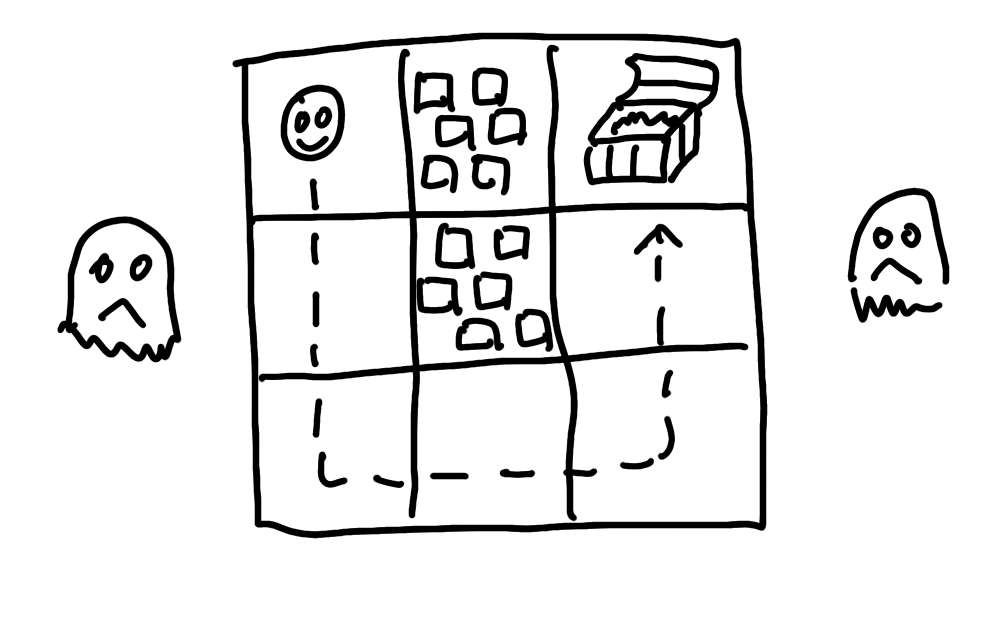
\includegraphics[width=35mm]{images/maze.png}};
\end{tikzpicture}

\end{frame}

\begin{frame}
  \centerline{Монадът Maybe}
\end{frame}


\begin{frame}[fragile]
  \frametitle{Maybe}

\begin{lstlisting}[basicstyle=\small,language=Haskell]
data Maybe a = Nothing | Just a

left :: Game -> Maybe Game
left (Game (x, y) w) 
    | dead w (x-1,y) = Nothing
    | otherwise = Just $ Game (x-1, y) w

\end{lstlisting}

\end{frame}


\begin{frame}[fragile]
  \frametitle{Обобщение на операциите}

\begin{lstlisting}[basicstyle=\small,language=Haskell]
move :: Game -> (Pos -> Pos) -> Maybe Game
move (Game p w) mv = if dead w (mv p) 
                     then Nothing 
                     else Just $ Game (mv p) w

left g = move g (\(x, y) -> (x-1, y))
right g = move g (\(x, y) -> (x+1, y))
up g = move g (\(x, y) -> (x, y-1))
down g = move g (\(x, y) -> (x, y+1))
\end{lstlisting}

\end{frame}


\begin{frame}[fragile]
  \frametitle{Разглеждане на случаи}

\begin{lstlisting}[basicstyle=\small,language=Haskell]
case val of
  pattern1 -> ...
  pattern2 -> ...
\end{lstlisting}

\end{frame}



\begin{frame}[fragile]
  \frametitle{Композиране на операции}

\begin{lstlisting}[basicstyle=\small,language=Haskell]
walk2 = case (down myWorld) of
             Nothing -> Nothing
             Just w -> case (down w) of
                        Nothing -> Nothing
                        Just w' -> case (right w') of
                                    Nothing -> Nothing
                                    Just w'' -> Just w''

\end{lstlisting}

\begin{itemize}
  \item А преди беше:
\end{itemize}

\begin{lstlisting}[basicstyle=\small,language=Haskell]
walk1 = myWorld->>down->>down->>right->>right->>up->>up
\end{lstlisting}


\end{frame}


\begin{frame}[fragile]
  \frametitle{Какво ни дават монадите?}

\begin{lstlisting}[basicstyle=\small,language=Haskell]
Just myWorld >>= down >>= down >>= right >>= 
     right >>= up >>= up
\end{lstlisting}

\begin{itemize}
  \item Дефиниция на \verb#>>=#
\end{itemize}

\begin{lstlisting}[basicstyle=\small,language=Haskell]
ghci>:info >>=
type Monad :: (* -> *) -> Constraint
class Applicative m => Monad m where
  (>>=) :: m a -> (a -> m b) -> m b
\end{lstlisting}
\end{frame}


\begin{frame}[fragile]
  \frametitle{Кака е дефиниранo това?}

\begin{lstlisting}[basicstyle=\small,language=Haskell]
--(>>=) :: m a -> (a -> m b) -> m b
instance Monad Maybe where
  ...
Nothing >>= f = Nothing
Just x >>= f = f x
\end{lstlisting}

\end{frame}


\begin{frame}[fragile]
  \frametitle{Какво са монадите?}

  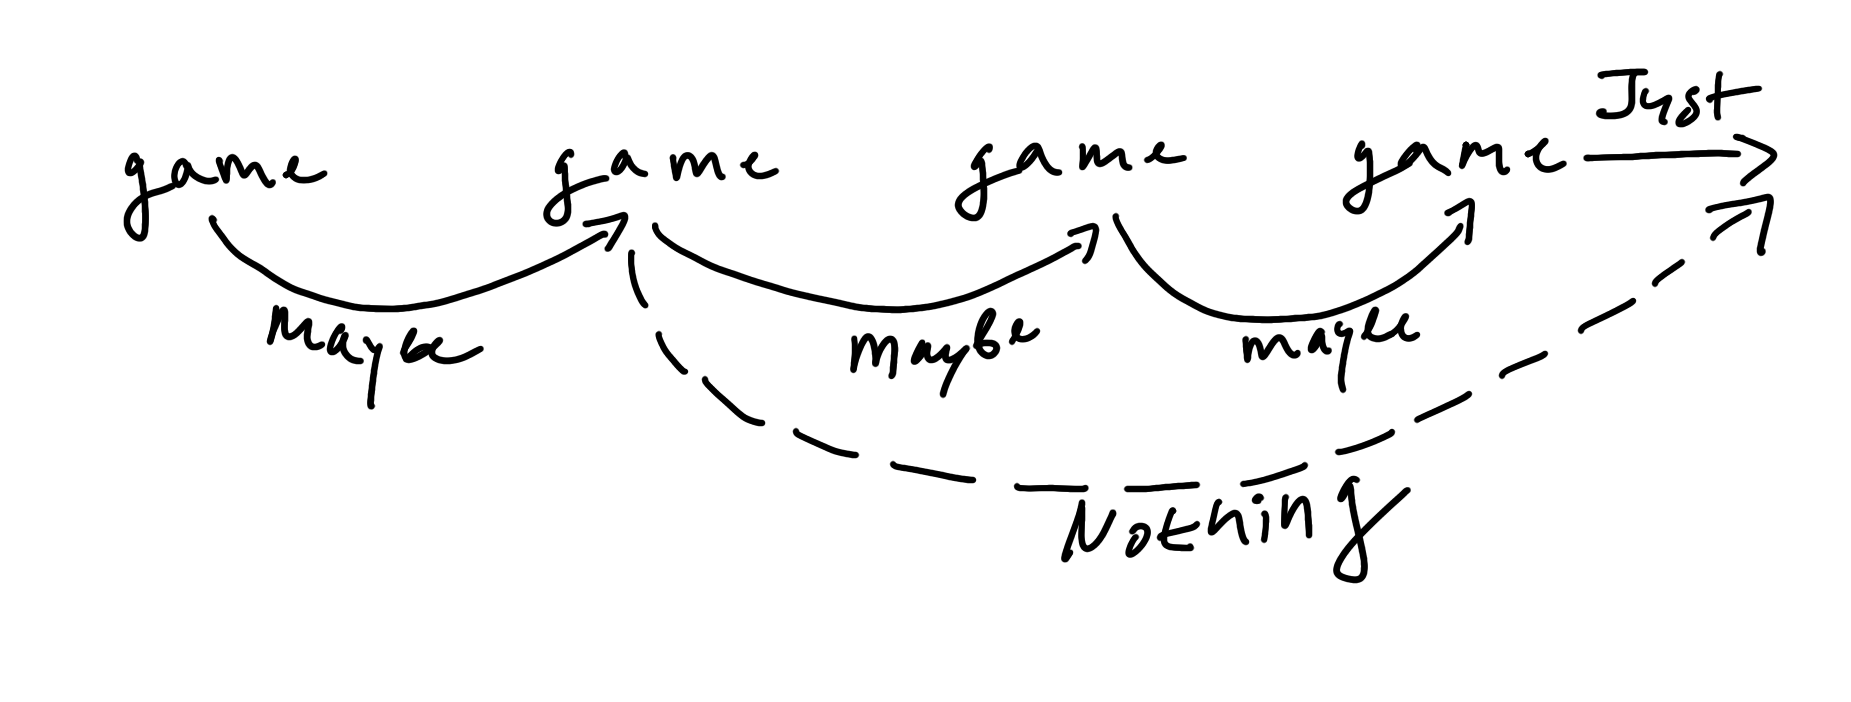
\includegraphics[width=110mm]{images/composition}

\begin{itemize}
  \item ``Закичват'' стойности с допълнителна информация (embelishment)
  \item Дефинират компизиция на операции
\end{itemize}

\end{frame}
 

\end{document}


\begin{columns}[t]
  \begin{column}{0.2\textwidth}

\relscale{0.63}
\begin{lstlisting}
\end{lstlisting}
\relscale{1}

  \end{column}
  \begin{column}{0.8\textwidth}

  \end{column}
\end{columns}


